\chapter[Landau-Ginzburg Effective Field Theory]{Landau-Ginzburg Effective \\Field Theory}

We are now ready to introduce the Landau-Ginzburg effective field theory, along with the field theory description of phase transitions. We will frame the discussion in the language of a magnetic system, with the simple Ising model as a paradigmatic example, but the discussion can be easily generalized to other systems and other order parameters.

The Landau-Ginzburg effective field theory is a \textbf{mesoscopic description} of phase transitions, which allows us to describe the behavior of the system near the critical point. Consider a ferromagnet such as iron, which can exhibit a phase transition from a paramagnetic to a ferromagnetic phase below a critical temperature $T_c$ (known as the \textit{Curie temperature}). Close to the critical point, we may expect that it is not necessary to know all the details about the microscopic costituent of the system and their interactions: indeed, as the correlation length diverges, the system becomes scale invariant, and the relevant degrees of freedom will become the collective excitations of the system, which are described by a mesoscopic parameters.

Therefore it makes sense to change paradigm from the microscopic description of the system, which is given by the Hamiltonian of the system, to a mesoscopic description, which will be given by a \textbf{free energy functional}. The mesoscopic degrees of freedom are much larger than the lattice spacing, but much smaller than the system size, so that they can be considered as continuous variables. We can thus imagine to define a field \(m(\mathbf{x})\) which gives the local average of the magnetization in a small region around the point \(\mathbf{x}\). The free energy functional will then be a functional of the field \(m(\mathbf{x})\), and it will encode the behavior of the system near the critical point.

\section{Mesoscopic Description of Phase Transitions}

Let us exemplify the concept of mesoscopic description of phase transitions by considering a trivial one dimensional chain of classical spins. Suppose the spins to be non interacting, so that the Hamiltonian of the system is simply given by the interaction with an external magnetic field \(h\):
\[
    H[\{s_i\}] = -h \sum_i s_i,
\]
and the partition function is given by
\[
    \mathcal{Z} = \sum_{\{s_i\}} e^{-\beta H[\{s_i\}]} = \sum_{\{s_i\}} e^{\beta h \sum_{i}  s_i} = {2 \cosh(\beta h)}^N.
\]

Let us now show how we can write the partition function in terms of a mesoscopic degrees of freedom. We can consider the groupings of \(M\) spins, with \(1 \ll M \ll N\), into \(N/M\) blocks of \(M\) spins each:
\[
    \cdots \underbracket{\uparrow \, \uparrow \, \downarrow \, \uparrow}_{\sigma_1 = 1/2}\, \underbracket{\downarrow \,\downarrow \, \uparrow \, \downarrow}_{\sigma_2 = -1/2}\, \underbracket{\uparrow \, \downarrow \, \downarrow \, \uparrow}_{\sigma_3 = 0}\, \underbracket{\uparrow \, \uparrow \, \uparrow \,\uparrow}_{\sigma_4 = 1} \cdots
\]
We associate to each block a mesoscopic degree of freedom \(\sigma_k\) defined as the average of the spins in the block:
\[
    \sigma_k = \frac{1}{M} \sum_{j = kM + 1}^{M(k+1)} s_j,
\]
which is not anymore a microscopic degree of freedom, since it is defined as an average over a block of spins, but instead a mesoscopic degree of freedom, since it is defined on a larger scale than the lattice spacing, but still very small compared to the system size. The variable \(\sigma_k\) can take values in the set \(\{-1, -1 + \frac{2}{M}, -1 + \frac{4}{M} \dots, 1 - \frac{4}{M}, 1 - \frac{2}{M}, 1\}\), which are the possible values of the average magnetization in a block of \(M\) spins.

Then we can rewrite the partition function as
\[
    \begin{aligned}
        \mathcal{Z} & = \sum_{\{s_i\}} e^{-\beta H[\{s_i\}]}                                                                                                                     \\
                    & = \sum_{\{\sigma_k\}} \sum_{\{s_i\}} \left[\prod_{k} \delta\left(\sigma_k - \frac{1}{M} \sum_{j = kM + 1}^{M(k+1)} s_j\right)\right] e^{-\beta H[\{s_i\}]} \\
                    & \eqqcolon \sum_{\{\sigma_k\}} e^{-\beta F[\{\sigma_k\}]},
    \end{aligned}
\]
where the second line is just a mathematical identity (since we inserted an integrated delta function), and we have defined the free energy functional \(F[\{\sigma_k\}]\) in the third line. Let us highlight the nature of the first summation: it goes over all the sequences
\[
    \{\sigma_k\}_{k=1}^{N/M}, \text{ with } \sigma_k \in \{-1, -1 + \tfrac{2}{M}, -1 + \tfrac{4}{M} \dots, 1 - \tfrac{4}{M}, 1 - \tfrac{2}{M}, 1\}.
\]
Thus, computing the functional \(F[\{\sigma_k\}]\) explicitly, we find
\[
    \begin{aligned}
        \mathcal{Z} & = \sum_{\{\sigma_k\}} \sum_{\{s_i\}} \left[\prod_{k} \delta\left(\sigma_k - \frac{1}{M} \sum_{j = kM + 1}^{M(k+1)} s_j\right)\right] e^{\beta h \sum_i s_i}                          \\
                    & = \sum_{\{\sigma_k\}} \sum_{\{s_i\}} \left[\prod_{k} \delta\left(\sigma_k - \frac{1}{M} \sum_{j = kM + 1}^{M(k+1)} s_j\right)\right] e^{\beta M h \sum_k \sigma_k}                   \\
                    & = \sum_{\{\sigma_k\}} e^{\beta M h \sum_k \sigma_k} \prod_k\left[ \sum_{\{s_j\}_{j=kM+1}^{M(k+1)}} \delta\left( \sigma_k - \frac{1}{M} \sum_{j = kM + 1}^{M(k+1)} s_j\right) \right] \\
                    & \eqqcolon \sum_{\{\sigma_k\}} e^{\beta M h \sum_k \sigma_k} \prod_k e^{S(\sigma_k)}                                                                                                  \\
                    & = \sum_{\{\sigma_k\}} e^{\beta M h \sum_k \sigma_k + \sum_k S(\sigma_k)} \eqqcolon \sum_{\{\sigma_k\}} e^{-\beta H[\{\sigma_k\}] + S[\{\sigma_k\}]},
    \end{aligned}
\]
where we have defined an entropic factor \(S(\sigma_k)\) as the logarithm of the number of configurations of the spins in the block \(k\) that give rise to a given value of \(\sigma_k\):
\[
    S(\sigma_k) = \log\left[\sum_{\{s_j\}_{j=kM+1}^{M(k+1)}} \delta\left( \sigma_k - \frac{1}{M} \sum_{j = kM + 1}^{M(k+1)} s_j\right)\right],
\]
and in the end we named
\[
    H[\{\sigma_k\}] = -M h \sum_k \sigma_k, \quad S[\{\sigma_k\}] = \sum_k S(\sigma_k).
\]
Now we can compute the entropic factor \(S(\sigma_k)\) explicitly. For \(\sigma = - 1 + \frac{2p}{M}\), with the correct values of \(p\) to make \(\sigma\) an allowed value, we have that the exponential of the entropy is given by the number of ways to choose \(p\) spins down in a block of \(M\) spins, which is given by the binomial coefficient \(\binom{M}{p}\). Thus we have
\[
    e^{S(\sigma)} = \binom{M}{p} = \binom{M}{\tfrac{M}{2}(\sigma + 1)} \implies S(\sigma) = \log\binom{M}{\tfrac{M}{2}(\sigma + 1)}.
\]

Putting everything together, we have that the partition function can be written in terms of the mesoscopic degrees of freedom \(\sigma_k\) as
\[
    \mathcal{Z} = \sum_{\{\sigma_k\}} e^{-\beta H[\{\sigma_k\}] + S[\{\sigma_k\}]} = \sum_{\{\sigma_k\}} e^{-\beta F[\{\sigma_k\}]}.
\]

\subsection{Principles and Free Energy Functional}

Thus we have found a way to write the partition function in terms of a mesoscopic degrees of freedom, and we have defined the free energy functional \(F[\{\sigma_k\}]\) as
\[
    F[\{\sigma_k\}] = H[\{\sigma_k\}] - \frac{1}{\beta} S[\{\sigma_k\}] = - M h \sum_k \sigma_k - \frac{1}{\beta} \sum_k \log\binom{M}{\tfrac{M}{2}(\sigma_{k} +1)}.
\]

In this simple case, the Hamiltonian \(H[\{\sigma_k\}]\) in terms of the collective variables \(\sigma_k\) has conserved the original functional form, with just a rescaling of the magnetic field \(h \to Mh\). However, the patition function has acquired a non trivial entropic contribution of the form \(S[\{\sigma_k\}] = \sum_k S(\sigma_k)\), which is a non trivial function of the mesoscopic degrees of freedom \(\sigma_k\). In general, it may not be as simple to find the explicit form of the free energy functional given any microscopic Hamiltonian, but in principle it is possible to do so by following the same procedure we have just outlined.

Close to criticality, we expect the density \(\sigma_k\) to vary smoothly across the system, allowing us to approximate the sequence \(\{\sigma_k\}\) with a continuous magnetization field \(m(\mathbf{x})\). We can then write the free energy functional as a functional of the continuous field \(m(\mathbf{x})\), where \(\mathbf{x}\) is the spatial coordinate in the system.
This is a mathematically delicate prcedure, which starts by identifying
\[
    m(\mathbf{x}) \simeq \frac{M \sigma_k}{\Delta x},
\]
which in a one dimensional system can be pictured as follows:
\begin{figure}[H]
    \centering
    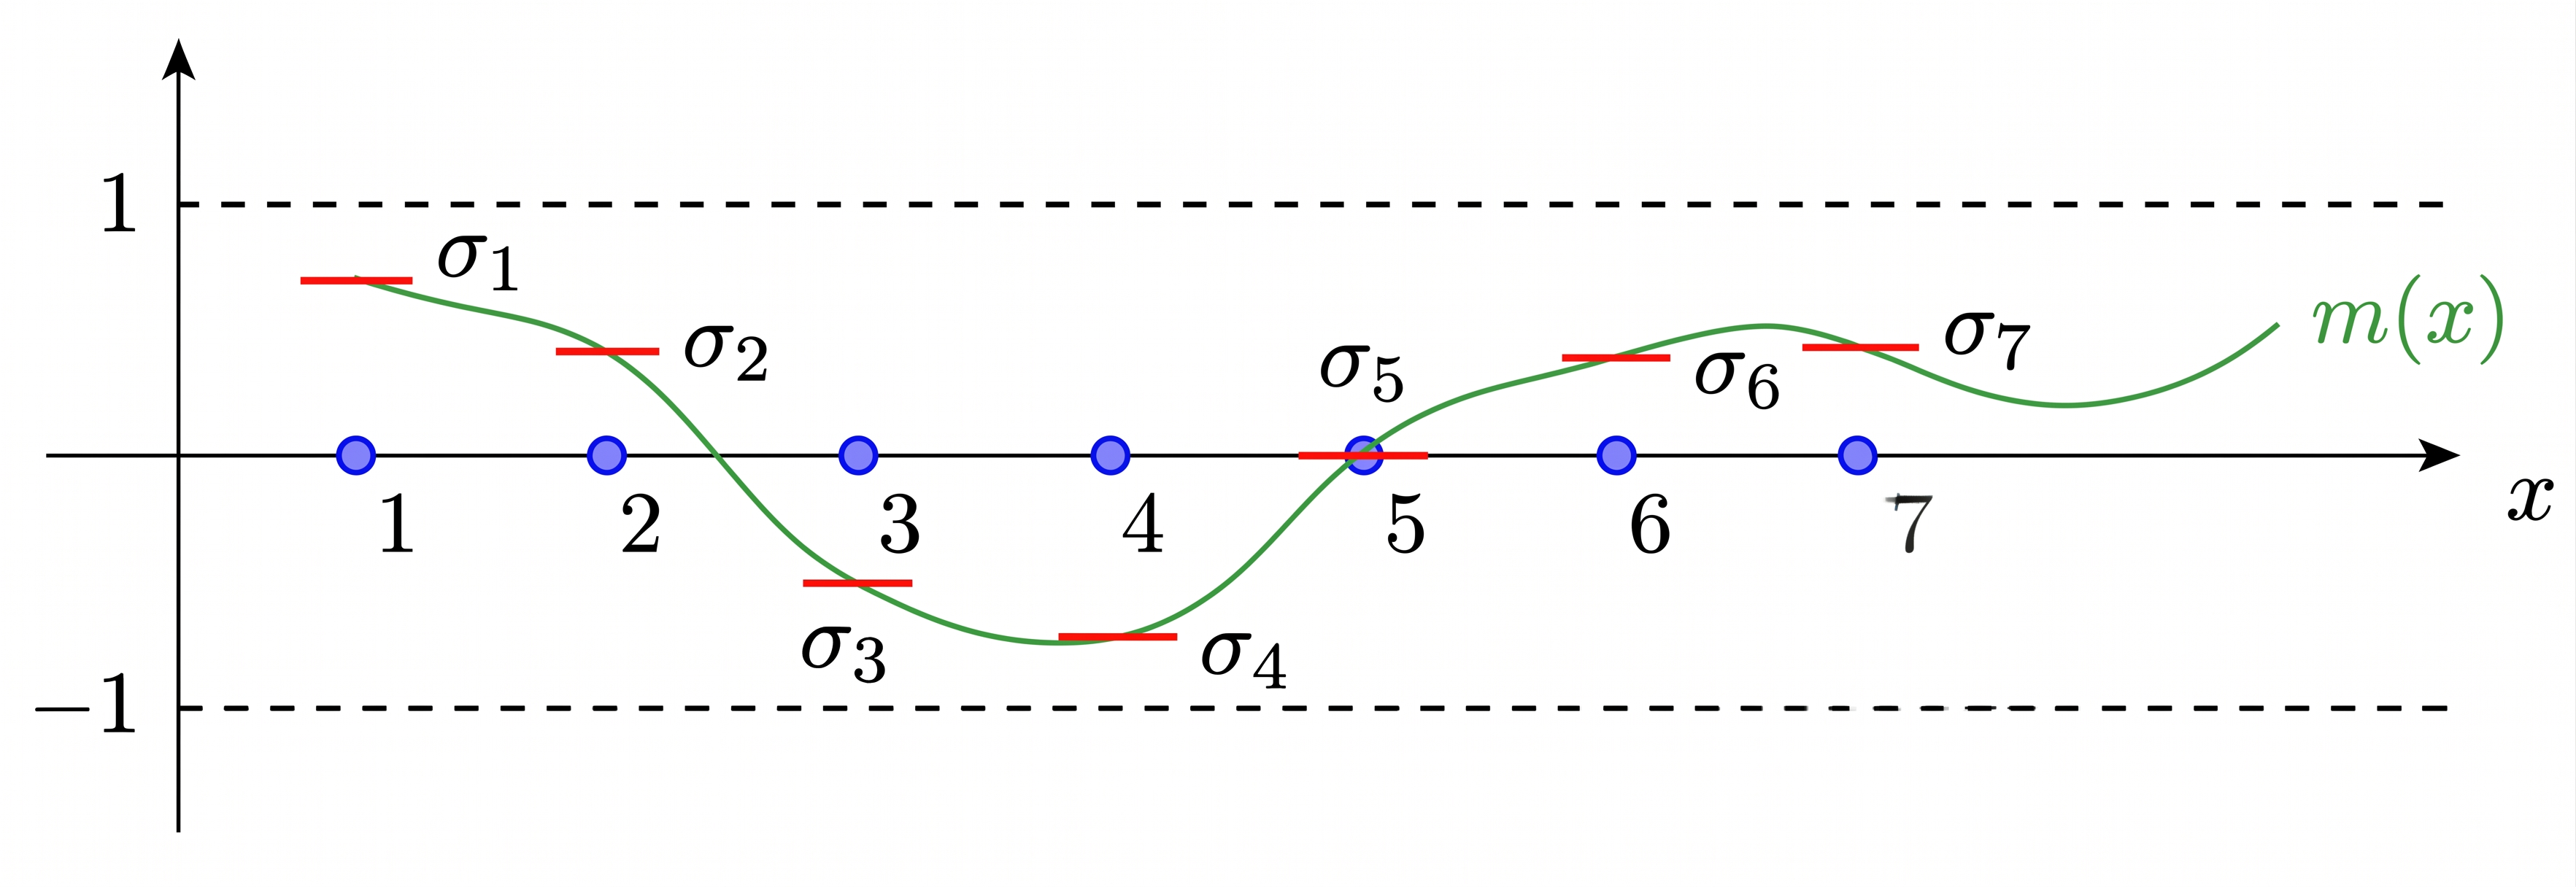
\includegraphics[width=0.8\textwidth]{img/LG_average_magnetization_field.png}
    \caption{Schematic representation of the \textit{coarse-graining procedure} in a one-dimensional system. The discrete mesoscopic degrees of freedom $\{\sigma_k\}$, defined on blocks of finite size $\Delta x$ and centered at $x_k$, are approximated by a continuous magnetization field $m(x)$ under the assumption that the magnetization varies slowly over spatial scales comparable to $\Delta x$.}
\end{figure}
The idea is to ``replace sum by integrals'' in the partition function, and to write the free energy functional as a functional of the continuous field \(m(\mathbf{x})\):
\[
    \sum_{k} \sigma_k = \sum_{k} \Delta x \frac{m(x_k)}{M} \simeq \frac{1}{M} \int \mathrm{d}^d \mathbf{x}\, m(\mathbf{x}),
\]
therefore letting us write the partition function as
\[
    \mathcal{Z} = \int \mathcal{D} m(\mathbf{x}) e^{-\beta F[m(\mathbf{x})]}.
\]
In general, finding the explicit form of the free energy functional \(F[m(\mathbf{x})]\) is a very difficult task, and it may not be possible to do so in a closed form. However, the LG theory gives us a prescription on how to describe it close to criticality, in terms of a few fenomenological parameters, by imposing some general principles on the form of the free energy functional.

The Landau-Ginzburg theory is very general. So far we have examined an uniaxial ferromagnet, where the order parameter is a scalar field \(m(\mathbf{x})\) that describes the local magnetization. In general, we can consider systems with phase transitions described by a vectorial order parameter field
\[
    \mathbf{m}(\mathbf{x}) \in \mathbb{R}^n, \text{ i.e. } \begin{dcases}
        \mathbf{x} = (x_1, \dots, x_d) \in \mathbb{R}^d, \\
        \mathbf{m}(\textbf{x}) = (m_1(\mathbf{x}), \dots, m_n(\mathbf{x})) \in \mathbb{R}^n,
    \end{dcases}
\]
where \(d\) is the spatial dimension and \(n\) is the number of components of the order parameter.

\begin{example}
    Taking in consideration some examples of other systems which can be described by the Landau-Ginzburg theory may help to clarify the generality of the theory:
    \begin{itemize}
        \item \((n=1)\): uniaxial ferromagnet, liquid-gas transition, binary mixtures, etc.
        \item \((n=2)\): superfluidity, superconductivity, planar magnets, etc.
        \item \((n=3)\): Heisenberg ferromagnet, classical magnets, etc.
    \end{itemize}
    Tipically, we consider systems in 3 spatial dimensions, so that \(d=3\), but it may happen to consider phase transitions appearing on surfaces, which are effectively two dimensional, or on lines, which are effectively one dimensional. In these cases, we will have \(d=2\) or \(d=1\) respectively.
\end{example}

\subsubsection{Landau-Ginzburg Prescription}

The Landau-Ginzburg theory gives us a prescription on how to describe the free energy functional \(F[m(\mathbf{x})]\) close to criticality, in terms of a few fenomenological parameters, by imposing some general principles on the form of the free energy functional. These principles are:
\begin{itemize}
    \item \textbf{Locality and uniformity}: different positions in the system are equivalent. Therefore, we must be abe to write the free energy functional as an integral in space of a free energy density \(\Phi(m(\mathbf{x}), \nabla m(\mathbf{x}), \dots)\) that depends on the field \(m(\mathbf{x})\) and its derivatives at the same point \(\mathbf{x}\):
          \[
              \beta F[m(\mathbf{x})] = \int \mathrm{d}^d \mathbf{x}\, \Phi(m(\mathbf{x}), \nabla m(\mathbf{x}), \nabla^2 m(\mathbf{x}), \dots),
          \]
          where integrating we are effectively removing the spatial dependence of the free energy functional.
    \item \textbf{Analiticity}: the function \(\Phi\) should be analytic in its arguments, since we do not expect any singularity in the free energy functional at mesoscopic scales (we are not at the critical point yet, where the correlation length diverges, but we are close to it). Close to criticality, the order parameter \(m(\mathbf{x})\) is small, so we can expand the free energy density \(\Phi\) in powers of \(m(\mathbf{x})\) and its derivatives, and keep only the leading terms in the expansion (we will later state this more precisely).
    \item \textbf{Symmetry}: the functional form of \(\Phi\) should reflect the symmetries of the model. In particular, a given term in the Taylor expansion of \(\Phi\) is allowed only if it does not break any of the symmetries of the model. For example, in the case of a uniaxial ferromagnet, the free energy functional should be invariant under the transformation \(m(\mathbf{x}) \to -m(\mathbf{x})\), since the system is symmetric under the inversion of the magnetization. This means that only even powers of \(m(\mathbf{x})\) are allowed in the expansion of \(\Phi\).
\end{itemize}

We now have all the ingredients to put the LG principle into pactice, and to write down the free energy functional close to criticality. We will do this in the next section, where we will apply the LG theory to the \(d\)-dimensional Ising model.

\subsection{Application on Ising Model}

Consider the \(d\)-dimensional Ising model, which is a generalization of the one-dimensional chain of classical spins we have considered before. Since the order parameter is a scalar mgnetization \(m \in \mathbb{R}\), we can follow the LG prescription and consider the scalar field \(m(\mathbf{x})\) (\(\mathbf{x} \in \mathbb{R}^d\)), the local (mesoscopic) magnetization. Thus we can build the mesoscopic partition function as a function of the field \(m(\mathbf{x})\) as
\[
    \mathcal{Z} = \int \mathcal{D} m(\mathbf{x}) e^{-\beta F[m(\mathbf{x})]},
\]
where we know
\[
    \beta F[m(\mathbf{x})] = \int \mathrm{d}^d \mathbf{x}\, \Phi(m(\mathbf{x}), \nabla m(\mathbf{x}), \nabla^2 m(\mathbf{x}), \dots).
\]

Close to the critical point, the configurations contribuiting the most to the partition function are those with small magnetization, so we can expand the free energy density \(\Phi\) in powers of \(m(\mathbf{x})\) and its derivatives, and keep only the leading terms in the expansion:
\[
    \Phi(m(\mathbf{x}), \nabla m(\mathbf{x}), \nabla^2 m(\mathbf{x}), \dots) = a_1 m(\mathbf{x}) + a_2 m^2(\mathbf{x}) + \dots + \sum_{k} b_k \partial_{x_k} m(\mathbf{x}) \dots
\]
The next prescription of the LG theory is to impose the symmetries of the model on the free energy density \(\Phi\). In the case of the Ising model, in the absence of the external field (\(h=0\)), the system is symmetric under a \(\mathbb{Z}_2\) transformation, mapped by \(m(\mathbf{x}) \to -m(\mathbf{x})\); thus only even powers of \(m(\mathbf{x})\) are allowed in the expansion of \(\Phi\), canceling out \(a_1\) as well as the other coefficients in front of odd powers. Thus we can write
\[
    \Phi [m(\mathbf{x}), \nabla m(\mathbf{x}), \nabla^2 m(\mathbf{x}), \dots] \big|_{h=0} = a_2 m^2(\mathbf{x}) + a_4 m^4(\mathbf{x}) + \dots + b_2 (\nabla m(\mathbf{x}))^2 + \dots
\]
Let us highlight that if we are in presence of the external field \(h\), the \(\mathbb{Z}_2\) symmetry is broken, and odd powers of \(m(\mathbf{x})\) are allowed in the expansion of \(\Phi\), but they must vanish with \(h\). Furthermore, close to criticality, even \(h\) has to be small, so we can keep terms linear in \(h\) in the expansion of \(\Phi\), and thus we can write
\[
    \begin{aligned}
        \Phi [m(\mathbf{x}), \nabla m(\mathbf{x}), \nabla^2 m(\mathbf{x}), \dots] & = a_2 m^2(\mathbf{x}) + a_4 m^4(\mathbf{x}) + \dots + b_1 (\nabla m(\mathbf{x}))^2 + \dots - h (m(\mathbf{x}) + \dots) \\
                                                                                  & \simeq \frac{t}{2} m^2(\mathbf{x}) + u m^4(\mathbf{x}) + \frac{\kappa}{2} (\nabla m(\mathbf{x}))^2 - h m(\mathbf{x}),
    \end{aligned}
\]
where we kept only a few of the first orders in the expansion, and we renamed the coefficients as \(a_2 = t/2\), \(a_4 = u\), \(b_1 = \kappa/2\), using conventional notation.

At this point, the parameters \(t\), \(u\) and \(\kappa\) are just phenomenological parameters, which depend on the microscopic details of the model, and in principle can also depend on the temperature \(T\). These are not universal parameters, and they should be fixed by experimental observations. One could also make assumptions based on the behavior of the system and the meaning of the powers associated to the parameters, but in the end these assumptions should be verified by experiments. For example, we can assume that \(u > 0\) in order to have a stable free energy functional, and we can also assume that \(t\) is a linear function of the temperature \(T\), such that \(t = 0\) at the critical temperature \(T_c\), so that \(t < 0\) for \(T < T_c\) and \(t > 0\) for \(T > T_c\). However, these assumptions may not hold in general.

Putting everything together, we have significantly simplified the problem of finding a form for the partition function close to criticality, by reducing it to the problem of finding a few phenomenological parameters \(t\), \(u\) and \(\kappa\) that describe the free energy functional:
\[
    \mathcal{Z} = \int \mathcal{D} m(\mathbf{x}) e^{-\int \mathrm{d}^d \mathbf{x}\, \left[ \frac{t}{2} m^2(\mathbf{x}) + u m^4(\mathbf{x}) + \frac{\kappa}{2} (\nabla m(\mathbf{x}))^2 - h m(\mathbf{x})\right]}.
\]
The price we have paid for this simplification is that we have lost the connection with the microscopic details of the model, and we have introduced some phenomenological parameters that need to be fixed by experiments: they have non trivial functional dependence on the temperature \(T\), the external field \(h\) and on the microscopic details of the model, and they are not universal parameters. However, the LG theory is very powerful, since it allows us to describe the behavior of the system close to criticality in terms of a few parameters.

\section{Saddle Point Approximation}

Continuing our study of the Landau-Ginzburg theory, let us report the form of the partition function we have found for the \(d\)-dimensional Ising model near criticality:
\[
    \mathcal{Z} = \int \mathcal{D} m(\mathbf{x}) e^{-\int \mathrm{d}^d \mathbf{x}\, \left[ \frac{t}{2} m^2(\mathbf{x}) + u m^4(\mathbf{x}) + \frac{\kappa}{2} (\nabla m(\mathbf{x}))^2 - h m(\mathbf{x})\right]}.
\]
Apart from the comment we already made about the phenomenological parameters \(t\), \(u\) and \(\kappa\), we can also notice that the partition function has a very appealing form: it is a \textbf{path integral}, which is one of the most studied objects in theoretical physics, and it is the starting point for many powerful techniques to study the behavior of the system close to criticality. Keep in mind that the exact evaluation is still far out of reach, thus making non-trivial to extract quantitative predictions from the partition function.

However, we can still extract some qualitative predictions from the partition function by making some approximations. The simplest approximation we can make is the \textbf{saddle point approximation}, which substantially consists in approximating the partition function by the contribution of the configuration \(m(\mathbf{x})\) that minimizes the free energy functional \(F[m(\mathbf{x})]\). This is a good approximation when the fluctuations around the minimum are small, which is typically the case far from criticality, where the correlation length is finite and the system is not scale invariant.

Let us first employ this approximation in a simple context, in order to get a better intuition on how it works, and then we will see how to generalize it to the case of the partition function we have found for the \(d\)-dimensional Ising model near criticality.

\begin{example}[Saddle Point Approximation: a simple integral]
    Let us consider the following simple integral:
    \[
        I = \int_a^b \mathrm{d}x\, e^{-R\,g(x)}, \quad R \in \mathbb{R},
    \]
    where we can suppose the parameer \(R\) to be large (\(R \gg 1\)) and \(g(x)\) to have a unique minimum at some point \(\overline{x} \in [a,b]\). In this way we can expand \(g(x)\) around the minimum \(\overline{x}\) as
    \[
        g(x) \sim g(\overline{x}) + \frac{1}{2} g''(\overline{x}) (x - \overline{x})^2 + \mathcal{O}((x - \overline{x})^3),
    \]
    where in the minimum we have \(g'(\overline{x}) = 0\) and \(g''(\overline{x}) > 0\). Thus we can write the integral as
    \[
        I \sim e^{-R\,g(\overline{x})} \int_a^b \mathrm{d}x\, e^{-\tfrac{R}{2} g''(\overline{x}) (x - \overline{x})^2} \sim e^{-R\,g(\overline{x})} \int_{-\infty}^{+\infty} \mathrm{d}x\, e^{-\tfrac{R}{2} g''(\overline{x}) (x - \overline{x})^2},
    \]
    where in the last step we have extended the limits of integration to infinity, since the main contribution to the integral comes from the region around the minimum \(\overline{x}\). The remaining integral is a Gaussian integral, which can be evaluated explicitly after the change of variable \(y = (x - \overline{x})\):
    \[
        I \sim e^{-R\,g(\overline{x})} \int_{-\infty}^{+\infty} \mathrm{d}y\, e^{-\tfrac{R}{2} g''(\overline{x}) y^2} = e^{-R\,g(\overline{x})} \sqrt{\frac{2\pi}{R\,g''(\overline{x})}}.
    \]
    If we now take the logarithm of the integral, we find
    \[
        \log I \sim -R\,g(\overline{x}) - \frac{1}{2} \log(R\,g''(\overline{x})) + \frac{1}{2} \log(2\pi) \sim -R\,g(\overline{x}) + \mathcal{O}(\log R),
    \]
    which means that up to subleading corrections in \(R\), the integral is dominated by the contribution of the minimum of the function \(g(x)\): we can replace the integral with the maximal value of the integrand, which is given by \(e^{-R\,g(\overline{x})}\)
    \[
        I = \int_a^b e^{-R\,g(x)} \sim e^{-R\,g(\overline{x})}.
    \]
    This is the essence of the saddle point approximation: the integral is dominated by the contribution of the minimum of the function \(g(x)\), and we can approximate the integral by the value of the integrand at the minimum, up to subleading corrections in \(R\). Of course, untill \(R\) remains finite, the saddle point approximation is not exact, but is a very powerful tool to extract qualitative predictions from the integral, and can be applied in many different contexts, such as the evaluation of path integrals, which is the case we are interested in.
\end{example}

\subsection{Application to the LG Ising Partition Function}

Thus we can apply the saddle point approximation to the partition function we have found for the \(d\)-dimensional Ising model near criticality, which is again given by
\[
    \mathcal{Z} = \int \mathcal{D} m(\mathbf{x}) e^{-\int \mathrm{d}^d \mathbf{x}\, \left[ \frac{t}{2} m^2(\mathbf{x}) + u m^4(\mathbf{x}) + \frac{\kappa}{2} (\nabla m(\mathbf{x}))^2 - h m(\mathbf{x})\right]}.
\]

Firstly, let us underline that the phenomenological parameter \(\kappa\) has to be positive: if it were negative, the free energy functional would not be stable, since it would be unbounded from below:
\[
    \Phi[m(\mathbf{x})] = \int \mathrm{d}^d \mathbf{x}\, \left[ \frac{t}{2} m^2(\mathbf{x}) + u m^4(\mathbf{x}) + \frac{\kappa}{2} (\nabla m(\mathbf{x}))^2 - h m(\mathbf{x})\right],
\]
we could choose an oscillating configuration of the field \(m(\mathbf{x})\) with a very large gradient, such that the contribution of the gradient term becomes very negative, and thus the free energy functional becomes unbounded from below, resulting in a divergence of the path-integral.

Thus we have to impose \(\kappa > 0\) in order to have a stable free energy functional, and the field configurations that maximize the previous integral is therefore constant in space
\[
    m(\mathbf{x}) = m, \quad \forall \mathbf{x} \in \mathbb{R}^d.
\]
Considering a system of finite size \(L\), the saddle point approximation gives us the following expression of the partition function:
\[
    \mathcal{Z} \simeq e^{-L^d \left[ \frac{t}{2} m^{*2} + u m^{*4} - h m^*\right]},
\]
where \(L^d = V\) is the volume of the system and we have defined \(m^*\) as the constant value of the field \(m(\mathbf{x})\) that minimizes the integral \(\Phi[m(\mathbf{x})]\).
Indeed, for a constant configuration of the field \(m(\mathbf{x})\), the contribution of the gradient term vanishes, and the integral reduces to
\[
    \Phi[m(\mathbf{x})=m] = V \left[ \frac{t}{2} m^2 + u m^4 - h m\right],
\]
Recognizing that this expression has the same functional form of the free energy density that we computed in the mean field approximation, we are not surprised since, as we will see, the saddle point approximation is a generalization of the mean field approximation.

In particular, the form of the free energy density depends on the sign of the parameter \(t\):
\begin{figure}[H]
    \begin{minipage}{0.45\textwidth}
        \centering
        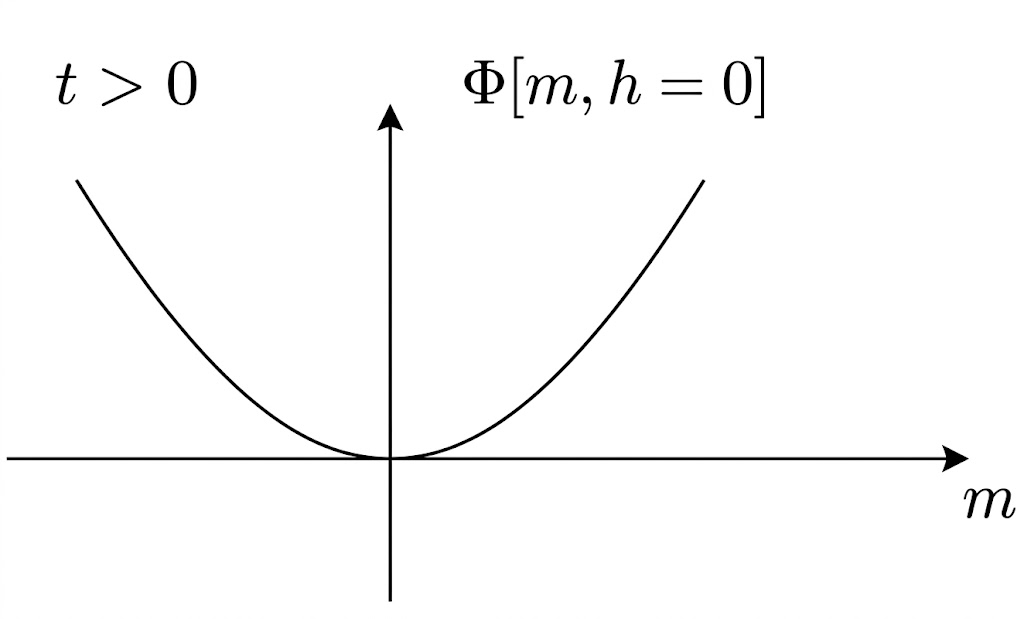
\includegraphics[width=0.8\textwidth]{img/spa_free_functional_t-g-0.jpg}
        \caption{Schematic representation of the free energy density \(\Phi(m)\) as a function of the magnetization \(m\) for \(t > 0\). In this case, the free energy density has a single minimum at \(m = 0\), which corresponds to the disordered phase of the system.}
    \end{minipage}
    \hfill
    \begin{minipage}{0.45\textwidth}
        \centering
        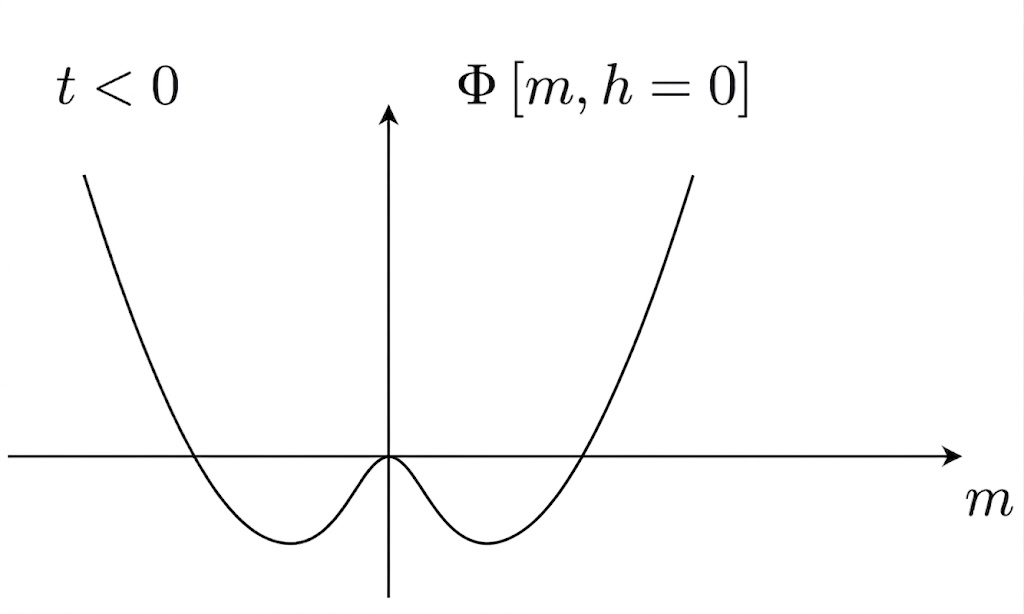
\includegraphics[width=0.8\textwidth]{img/spa_free_functional_t-l-0.jpg}
        \caption{Schematic representation of the free energy density \(\Phi(m)\) as a function of the magnetization \(m\) for \(t < 0\). In this case, the free energy density has two symmetric minima at \(m = \pm m^*\), which correspond to the ordered phase of the system. The minimum at \(m = 0\) becomes a local maximum, indicating that the disordered phase is unstable.}
    \end{minipage}
\end{figure}

Thus, it is natural to postulate the following functional dependence of the parameter \(t\) on the temperature \(T\):
\[
    t(T) = a (T - T_c) + \mathcal{O}((T - T_c)^2),
\]
since we want \(t\) to vanish at the critical temperature \(T_c\), and to be positive for \(T > T_c\) and negative for \(T < T_c\). With this assumption, we can see that the system undergoes a phase transition at the critical temperature \(T_c\), where the free energy density changes its shape, going from a single minimum at \(m = 0\) for \(T > T_c\) to two symmetric minima at \(m = \pm m^*\) for \(T < T_c\).

With this identification, we have fully recovered the mean field approximation for the Ising model, and its predictions. Thus it is now clear that \uline{the mean field approximation is a particular case of the saddle point approximation}, where we restrict the field configurations to be constant in space, and we look for the value of the constant field that minimizes the free energy functional. The saddle point approximation is a generalization of the mean field approximation, since it allows us to consider non-constant configurations of the field \(m(\mathbf{x})\), and thus to take into account spatial fluctuations of the order parameter.

Now in principle, we could go back to the path integral and \uline{estimate the corrections to the saddle point approximation by considering \textbf{field fluctuations} around the minimum of the free energy functional}.

\subsection{Lower and Upper Critical Dimension}

Let us underline the substantial difference between the first simple example of the saddle point approximation we have considered, which is a simple integral, and the second example, which is a path integral.
\begin{itemize}
    \item In the first case, the saddle point approximation is a good approximation when the parameter \(R\) is large, since in this case the fluctuations around the minimum of the function \(g(x)\) are suppressed by the factor \(R\) in the exponent.
    \item In the second case, we did not use any ``large parameter'' to justify the saddle point approximation, and it is still not clear at the moment under which conditions the saddle point approximation is a good approximation near criticality. In the next section, we will see how this is exactely done estimating the fluctuations around the minimum of the free energy functional, and we will find that \uline{the validity of the saddle point approximation depends on the spatial dimension \(d\) of the system}.
\end{itemize}
In particular, we will find that there exists a \textbf{lower critical dimension} \(D_l\) and an \textbf{upper critical dimension} \(D_c\) such that:
\begin{itemize}
    \item For \(d < D_l\), the SPA gives wrong predictions.
    \item For \(D_l < d < D_c\), there may be some divergences in the corrections to the SPA, but the qualitative predictions of the SPA are still correct; the same cannot be said for quantitative results, which are modified by the fluctuations around the minimum of the free energy functional.
    \item For \(d > D_c\), the fluctuations around the minimum of the free energy functional are weak enough that they do not modify the critical behavior of the system, resulting in a correctness of the SPA both qualitatively and quantitatively: the critical exponents predicted by the SPA are exact for \(d > D_c\).
\end{itemize}

In the case of the Ising model, we will find that the lower critical dimension is \(D_l = 1\) and the upper critical dimension is \(D_c = 4\). This means that the SPA gives wrong predictions for the one-dimensional Ising model (for which we have an analytical solution), it gives correct qualitative predictions but wrong quantitative predictions for the two- and three-dimensional Ising model,\footnote{The qualitative structure of the phase diagram is correct, but the quantitative values of the critical exponents are modified by fluctuations in the mean field approximation (which, as we have already seen, is just a particular case of the saddle point approximation).} and it gives correct qualitative and quantitative predictions, giving us the exact critical exponents.

Before proceeding, let us summarize the emergent picture of a generic continuous phase transition that we have obtained so far:
\begin{itemize}
    \item The system undergoes a continuous phase transition at the critical temperature \(T_c\), where the free energy density changes its shape, describing a transition from a disordered phase to an ordered one.
    \item Above the critical temperature \(T_c\), the system is in a disordered phase, and it is invariant under the action of a certain symmetry group \(G\) (for example, in the case of the Ising model, the system is invariant under a \(\mathbb{Z}_2\) transformation).
    \item Under the critical temperature \(T_c\), the system is in an ordered phase, and \textbf{the symmetry} \(G\) \textbf{is spontaneously broken}, since the system chooses one of the minima of the free energy density, which are not invariant under the action of the symmetry group \(G\): an \textbf{order parameter} \(m\) emerges, which is zero in the disordered phase and non-zero in the ordered phase, and which transforms non-trivially under the action of the symmetry group \(G\).
    \item Based on physical principles, one can describe the behaviour of this order parameter at mesoscopic scales by a \textbf{free energy functional} \(F[m(\mathbf{x})]\), with the \textit{path integral formulation of the LG theory}.
    \item At the zeroth order, we can apply the \textbf{saddle point approximation} to the partition function, which can gives us the mean field approximation for the system, and allows us to extract some qualitative predictions (exact if \(d > D_c\)) about the behavior of the system close to criticality.
\end{itemize}

In the following, we will complete our study of LG theory by analyzing the fluctuations. This will allow us to determine the upper critical dimension for the Ising model (note that we have previously established $D_l = 1$, based on its exact solution). Before embarking on this, let us show that, even when working at the level of the saddle-point approximation, the LG free-energy contains more information than the mean-field approach, as the LG theory takes into account the spatial dependence: we will be able to describe non-uniform configurations of the order parameter, which are not captured by the mean-field approximation, and which are relevant for the description of phenomena such as domain walls, interfaces, and critical fluctuations.

\subsection{Domain Walls}

Taking again into consideration the Ising model in \( d \) dimensions in the ordered phase (\( t < 0 \)) and \textbf{fix the boundary conditions} \( m(x_1 \to \pm\infty) = \pm\overline{m} \), where \( x_1 \) is the first coordinate of the position vector \( \mathbf{x} = (x_1, \dots, x_d) \). Here, \( \pm\overline{m} \) are the two equilibrium values at temperature \( t \). Let us use LG theory along with the saddle-point approximation to predict the spatial dependence of \( m(\mathbf{x}) \) in this setting: we want to find the configuration of the field \( m(\mathbf{x}) \) that minimizes the free energy functional, given the boundary conditions we have imposed. This configuration will describe a \textbf{domain wall}, which is a non-uniform configuration of the order parameter that interpolates between the two equilibrium values \( -\overline{m} \) and \( +\overline{m} \) across space.

The starting point is the LG partition function we previously derived for the \(d\)-dimensional Ising model near criticality, which is given by
\[
    \mathcal{Z} = \int \mathcal{D}m(\mathbf{x}) e^{-\int \mathrm{d}^d \mathbf{x} \left[ \frac{t}{2}m^2(\mathbf{x}) + u m^4(\mathbf{x}) + \frac{\kappa}{2}(\nabla m)^2 - h m(\mathbf{x}) \right]} ,
\]
where now the path integral is only over functions \( m(\mathbf{x}) \) such that
\[
    \lim_{x_1 \to \pm\infty} m(x_1, x_2 \dots x_d) = \pm\overline{m} .
\]

We now apply the saddle-point approximation. However, the minimum of the free energy is not given by \( m(\mathbf{x}) \) constant, because this does not satisfy the boundary condition (it has to give two opposite values at the boundaries, therefore it cannot be constant).
To find the correct minimum, we need to take a \underline{functional derivative} of the free energy. This is a tool in functional analysis which generalizes the derivative, and it is used, for instance, to derive the Euler-Lagrange equations of statistical mechanics from the least-action principle. To see how it works, take a field configuration \( m(\mathbf{x}) \) and perturb it by a small amount
\[
    m(\mathbf{x}) \mapsto m(\mathbf{x}) + \delta m(\mathbf{x}), \text{ with } \delta m(\mathbf{x}) = 0 \text{ at the boundaries} .
\]
The change in the LG free energy (up to \( O(\delta m(\mathbf{x})) \)) can be computed by inserting the variation of the field configuration into the free energy functional and expanding to first order in \( \delta m(\mathbf{x}) \): we are computing the functional derivative of the free energy functional with respect to the field \( m(\mathbf{x}) \)
\[
    \begin{aligned}
        \delta \left[ \int \mathrm{d}^d \mathbf{x} \left[ \frac{t}{2} m^2(\mathbf{x}) + u m^4(\mathbf{x}) + \frac{\kappa}{2}(\nabla m)^2 \right] \right] \\
        = \int \mathrm{d}^d \mathbf{x} \left[ t m(\mathbf{x}) \delta m(\mathbf{x}) + 4 u m^3(\mathbf{x}) \delta m(\mathbf{x}) + \kappa (\nabla m) \cdot \nabla(\delta m) \right],
    \end{aligned}
\]
where now the last term can be integrated by parts to give
\[
    \int \mathrm{d}^d \mathbf{x} (\nabla m) \cdot \nabla(\delta m) = - \int \mathrm{d}^d \mathbf{x} (\nabla^2 m) \delta m + \underbrace{\int \mathrm{d}^d \mathbf{x} \nabla \cdot (\nabla m \delta m)}_{(*)}.
\]
We have \( (*) = 0 \), since we choose \( \delta m(\mathbf{x}) = 0 \) at the boundary of the
integration domain. Therefore, substituting back into the previous expression, we find
\[
    \begin{aligned}
        \delta \left[ \int \mathrm{d}^d \mathbf{x} \left[ \frac{t}{2} m^2(\mathbf{x}) + u m^4(\mathbf{x}) + \frac{\kappa}{2}(\nabla m)^2 \right] \right] \\
        = \int \mathrm{d}^d \mathbf{x} \left[ t m(\mathbf{x}) + 4 u m(\mathbf{x})^3 - \kappa \nabla^2 m(\mathbf{x}) \right] \delta m(\mathbf{x}).
    \end{aligned}
\]
The saddle-point condition is \( \delta F / \delta m(\mathbf{x}) = 0 \), which finally gives
\[
    \kappa \nabla^2 m(\mathbf{x}) = t m(\mathbf{x}) + 4 u m(\mathbf{x})^3.
\]
These are the \textbf{Euler-Lagrange equations} for our field theory.

Coming back to our problem, we can reduce the Euler-Lagrange equations to a 1D equation (since we are only considering spatial variation along \( x_1 \)) giving
\[
    \kappa \frac{\mathrm{d}^2}{\mathrm{d}x^2} m(x) = t m(x) + 4 u m(x)^3
\]
where we renamed \( x_1 = x \). Using
\[
    \frac{\mathrm{d}^2}{\mathrm{d}x^2} \tanh(ax) = a^2 \tanh(ax)[1 - \tanh^2(ax)]
\]
we find the solution from the previous equation, which is given by
\[
    m(x) = \overline{m} \tanh\left(\frac{x - x_0}{w}\right),
\]
where
\[
    w = \sqrt{\frac{2 \kappa}{-t}}, \quad \overline{m} = \sqrt{\frac{-t}{4 u}},
\]
are the \textbf{width of the domain wall} and the equilibrium value of the magnetization, respectively.
\begin{figure}[H]
    \centering
    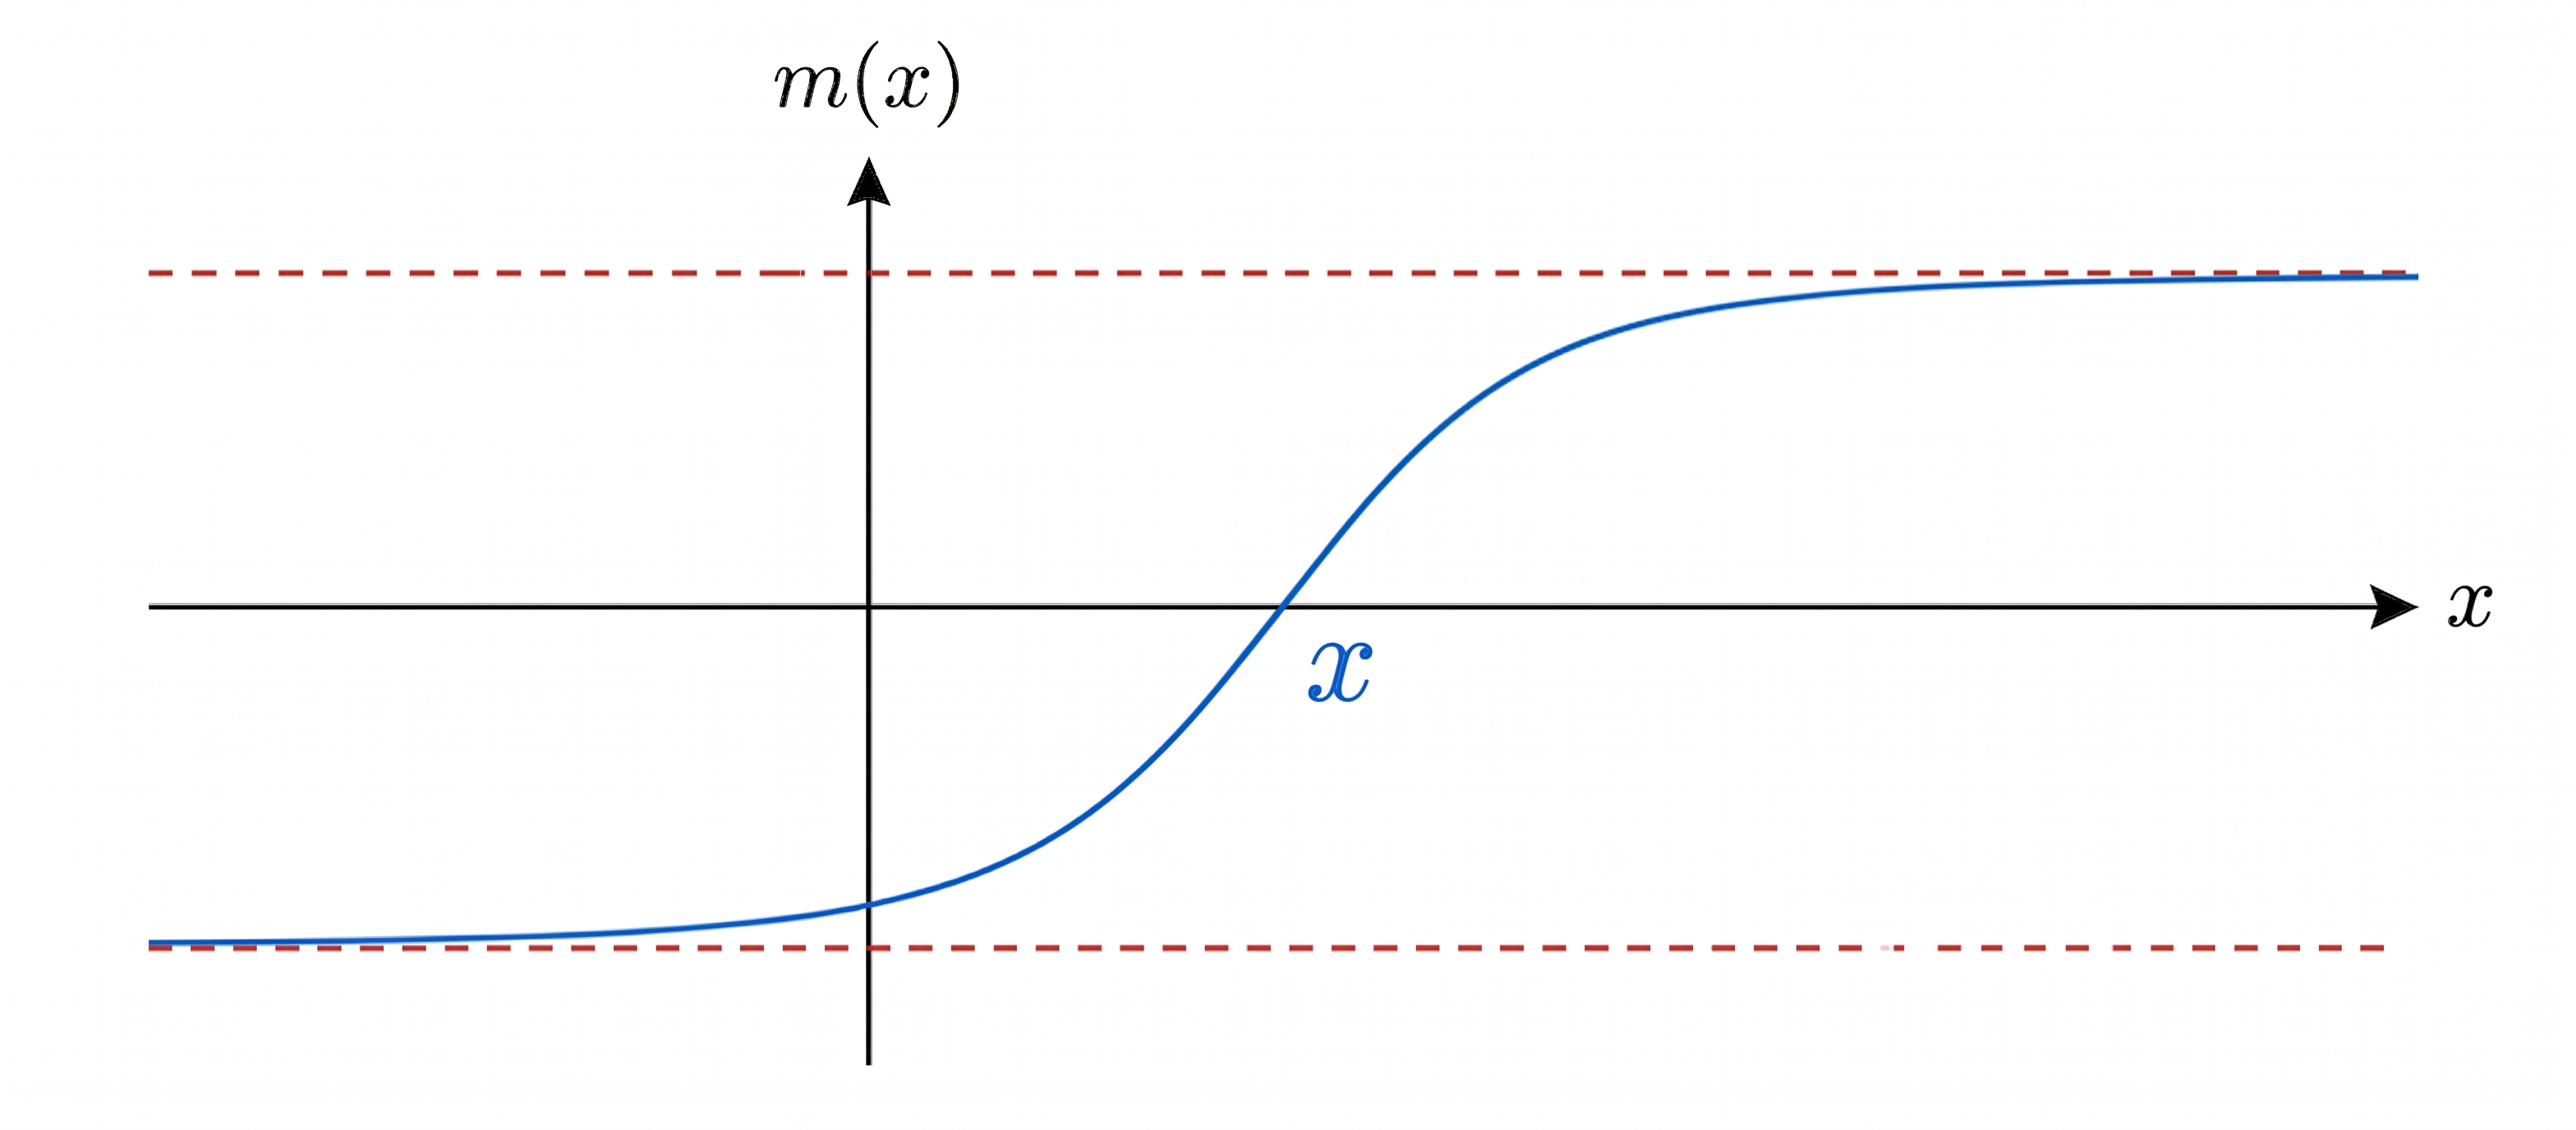
\includegraphics[width=0.8\textwidth]{img/spa_domain_wall.png}
    \caption{Schematic representation of the spatial dependence of the magnetization field \(m(x)\) in the presence of a domain wall, as predicted by the Landau-Ginzburg theory. The magnetization field \(m(x)\) interpolates smoothly between the two equilibrium values \(-\overline{m}\) and \(\overline{m}\) across a region of finite width \(w\), which characterizes the domain wall. The position of the domain wall is given by the free parameter \(x_0\).}
\end{figure}
Here \(x_0\) is a free parameter, which represents the position of the domain wall, that emerges between \(-\overline{m}\) at \(x=-\infty\) and \(\overline{m}\) at \(x=+\infty\). The width of the domain wall is given by \(w\), which diverges as we approach the critical temperature \(T_c\) (where \(t \to 0^-\), we will see this more clearly later). This is a manifestation of the critical fluctuations that occur near the phase transition, and it is a feature that cannot be captured by the mean-field approximation, which predicts a sharp domain wall with zero width.

Thus we were able to find a non-uniform configuration of the order parameter \(m(\mathbf{x})\) that minimizes the free energy functional, and which describes a domain wall. This is an example of how the Landau-Ginzburg theory allows us to describe phenomena that are not captured by the mean-field approximation, by taking into account the spatial dependence of the order parameter and its fluctuations. The mean-field approximation, on the other hand, would predict a sharp domain wall with zero width, which is not physical and does not capture the critical fluctuations that occur near the phase transition.